%BEGIN TICKET 21
\begin{properties}[несобственных интегралов]
    \begin{enumerate}
        \item Аддитивность. Пусть $f \in C[a, b)$,  $c \in (a, b)$. Если  $\int\limits_a^b f$ сходится, то  $\int\limits_c^b f$ сходится и  $\int\limits_a^b f = \int\limits_a^c f + \int\limits_c^b f$.
        \item Если $\int\limits_a^b f$ сходится, то  $\lim\limits_{c \to b-} \int\limits_c^b f = 0$
        \item Линейность $\alpha, \beta \in \R$ и $\int\limits_a^b f$ и  $\int\limits_a^b g$ сходятся. Тогда  $\int\limits_a^b(\alpha f + \beta g)$ сходится и $\int\limits_a^b (\alpha f + \beta g) = \alpha \int\limits_a^b f + \beta\int\limits_a^b g$.
        \item Монотонность. Пусть $\int\limits_a^b f$ и $\int\limits_a^b g$ существуют в  $\overline{R}$ и  $f \le g$ на $[a, b)$. Тогда  $\int\limits_a^b f \le \int\limits_a^b g$.
        \item Интегрирование по частям. $f, g \in C^1[a; b) \implies \int\limits_a^b fg' = fg \Big|_a^b - \int\limits_a^b f'g$.
        \item Замена переменных. $\vphi\!: [\alpha, \beta) \to [a, b)$,  $\vphi \in C^1[\alpha, \beta)$ и $\exists \lim\limits_{\gamma \to \beta-} \vphi(\gamma) \eqqcolon \vphi(\beta-)$ и $f \in C[a, b)$.

            Тогда  $\int\limits_\alpha^\beta f(\vphi(t)) \vphi'(t)\mathrm{d}t = \int\limits_{\vphi(\alpha)}^{\vphi(\beta-)} f(x) \mathrm{d}x$. <<Если существует один из  $\int$, то существует второй и они равны>>
    \end{enumerate}
\end{properties}
\begin{proof}
    \begin{enumerate}
        \item $\int\limits_a^b f = \lim\limits_{B \to b-} F(B) - F(a) \implies \lim_{B \to b-}F(B)$ существует и конечен  $\implies \int\limits_c^b = \lim\limits_{B \to b-} F(b) - F(c)$ --- сходится ($F(c)$ --- просто число какое-то).

            $\int\limits_a^b = \lim F(B) - F(a) = \lim F(B) - F(c) + F(c) - F(a) = \int\limits_c^b f + \int\limits_a^c f$.
        \item $\int\limits_c^b f = \int\limits_a^b f- \color{blue}{\int\limits_a^c f \underset{c \to b-}{\to} \int\limits_a^b f} \Rightarrow$ разность $\to 0$
        \item $\int\limits_a^b (\alpha f + \beta g) = \lim\limits_{B \to b-} \int\limits_a^B(\alpha f + \beta g) = \lim\limits_{B \to b-}(\alpha \int\limits_a^B f + \beta \int\limits_a^B g) = \alpha \lim\limits_{B \to b-} \int\limits_a^B f + \beta\lim\limits_{B \to b-} \int\limits_a^B g = \alpha \int\limits_a^b f + \beta \int\limits_a^b g$.
        \item $\int\limits_a^B f \le \int\limits_a^B g$ (монотонность собственных интегралов), а дальше предельный переход:\\
        $\lim\limits_{B \to b-} \int\limits_a^B f \le \lim\limits_{B \to b-} \int\limits_a^B g$
        \item $a < B < b$ и пишем формулу интегрирования по частям: $\int\limits_a^B fg' = fg \Big|_a^B - \int\limits_a^B f'g$ и переходим к пределу при $B \to b-$. Так как $f, g$ --- непрерывные функции, то  $\lim\limits_{B \to b-} fg\Big|_a^B = fg \Big|_a^b$ и получаем, что нужно.
        \item $F(y) \coloneqq \int\limits_{\vphi(\alpha)}^y f(x) \mathrm{d}x$,  $\Phi(\gamma) \coloneqq \int_{\alpha}^{\gamma} f(\vphi(t)) \vphi'(t) \mathrm{d}t$. Знаем, что $F(\vphi(\gamma)) = \Phi(\gamma)$ при  $\alpha < \gamma < \beta$.

            Пусть существует правый  $\int$, то есть  $\exists \lim\limits_{y \to \vphi(\beta-)} F(y)$. Возьмем  $\gamma_n \nearrow \beta \implies \vphi(\gamma_n) \to \vphi(\beta-) \implies \Phi(\gamma_n) = F(\vphi(\gamma_n)) \to \int\limits_{\vphi(\alpha)}^{\vphi(\beta-)} f(x) \mathrm{d}x$. При этом $\Phi(\gamma_n) \to \int\limits_{\alpha}^{\beta} f(\vphi(t))\vphi'(t)\mathrm{d}t$.

            Пусть существует левый $\int$, то есть  $\exists \lim\limits_{\gamma \to \beta-} \Phi(\gamma)$. Докажем, что  $\exists$ правый  $\int$. При  $\vphi(\beta-) < b$ нечего доказывать. 

            Пусть  $\vphi(\beta-) = b$. Тогда  возьмем $b_n \nearrow b$. Можно считать, что $b_n \in [\vphi(\alpha), b)$. Тогда $\exists \gamma_n \in [\alpha, \beta)\!: \vphi(\gamma_n) = b_n$. Докажем, что  $\gamma_n \to \beta$. Пусть это не так. Тогда найдется  $\gamma_{n_k} \to \widetilde{\beta} < \beta \implies \vphi(\gamma_{n_k}) \to \vphi(\widetilde{\beta}) < b$ по непрерывности $\vphi$ в точке $\widetilde{\beta}$. Противоречие.

            Итак,  $\gamma_n \to \beta$,  $F(b_n) = F(\vphi(\gamma_n)) = \Phi(\gamma_n) \to \int\limits_\alpha^\beta f(\vphi(t))\vphi'(t) \mathrm{d}t$.
    \end{enumerate}
\end{proof}
\begin{remark}[к третьему свойству]
    \begin{enumerate}
        \item Если  $\int\limits_a^b f$ сходится, а  $\int\limits_a^b g$ расходится, то  $\int\limits_a^b (f+g)$ расходится. Доказательство от противного, пусть интеграл сходится, тогда  $g = (f+g)-f \implies \int\limits_a^b g$ сходится.
        \item Если $\int\limits_a^b f$ и  $\int\limits_a^b g$ расходятся, то  $\int\limits_a^b (f+g)$ может сходиться.  $\int\limits_1^{+\infty} \frac{\mathrm{d}x}{x}$ и $\int\limits_1^{+\infty} -\frac{\mathrm{d}x}{x}$ расходятся.
    \end{enumerate}
\end{remark}
\begin{remark}[к шестому свойству]
    $\int\limits_a^b f(x) \mathrm{d}x$. Сделаем замену  $x = b - \frac{1}{t} = \vphi(t)$, $\vphi'(t) = \frac{1}{t^2}, \vphi(\alpha) = a, \alpha = \frac{1}{b-a}$.

    Тогда $\int\limits_a^b f(x) \mathrm{d}x = \int\limits_{\frac{1}{b-a}}^{+\infty} f(b-\frac{1}{t}) \frac{1}{t^2} \mathrm{d}t$.
\end{remark}

\begin{definition}
    Пусть $f$ непрерывна на  $(a, b)$ за исключением некоторого количества точек  $c_1 < c_2 < \ldots < c_n$.

    $\int\limits_a^b f$ сходится, если сходятся интегралы по всем маленьким отрезкам (содержащим только одну выколотую точку).
     \begin{figure}[h!]
    	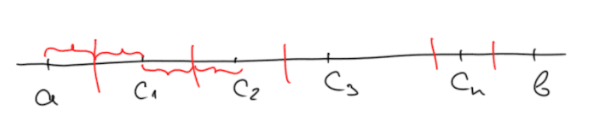
\includegraphics[scale=0.6]{improper}
    \end{figure}
\end{definition}
%END TICKET 21